\hyphenation{
Schnitt-stel-le
}
\paragraph{Praxisbeispiele} In diesem Abschnitt werden drei Beispiele für Dateiablagen vorgestellt, die aus Baden-Württemberg, Hamburg und Österreich stammen. Das Landesdenkmalamt von Baden-Württemberg verwendet eine Dateiablage, die an der analogen Ordnerstruktur einer Grabung orientiert ist. Sie wird in Abbildung \ref{OrdnerstrukturBaWue} veranschaulicht.

\begin{figure}[h!tb]
  \begin{center}
    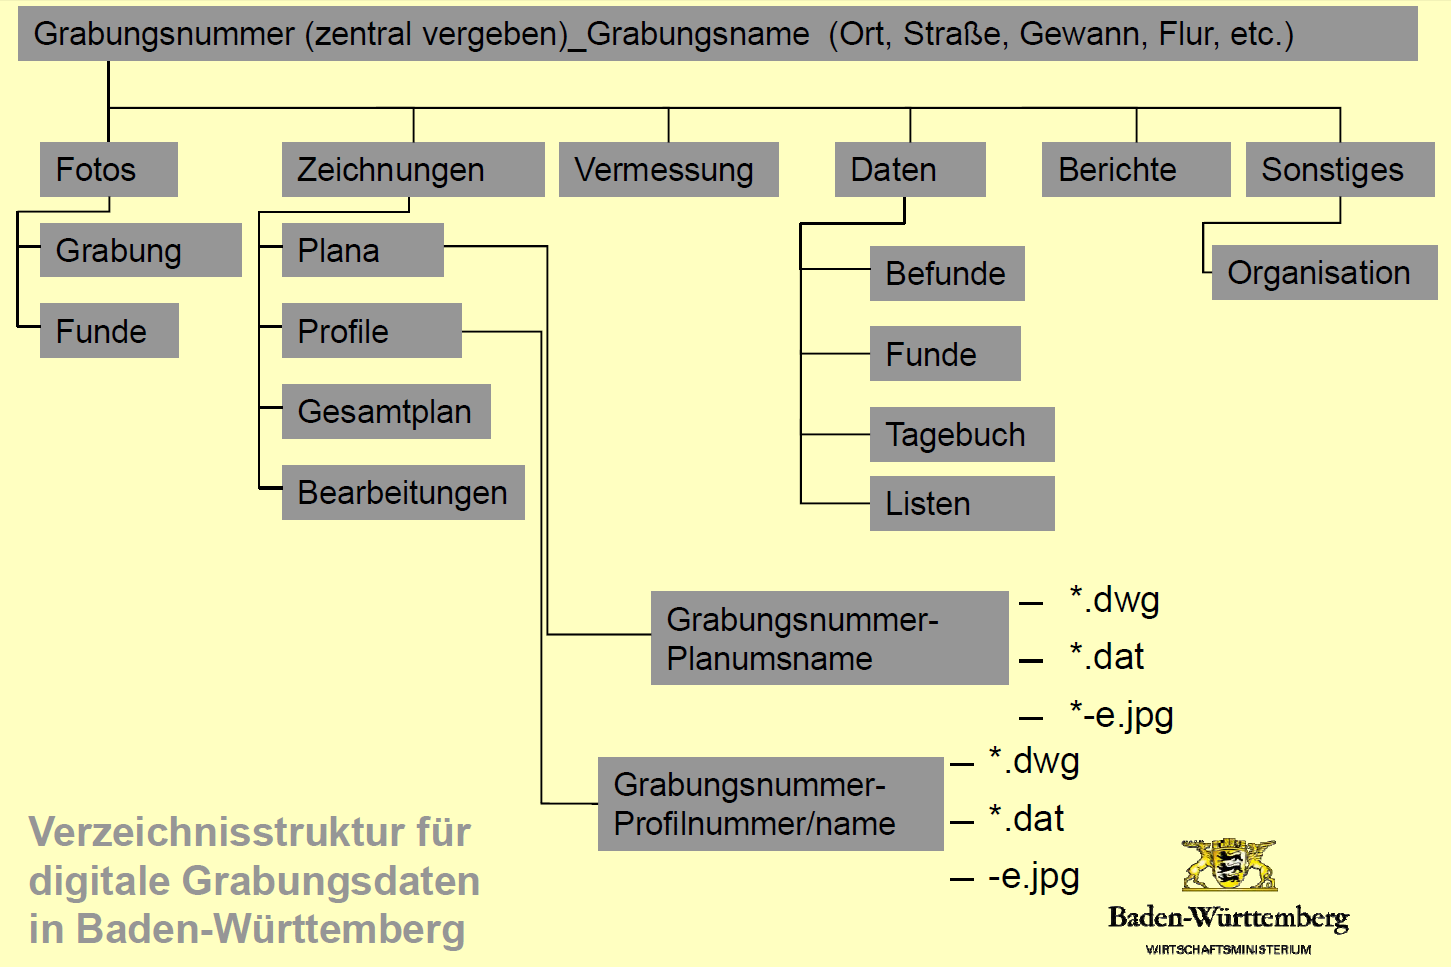
\includegraphics[width=0.9\textwidth]{bilder/OrdnerstrukturBaWue_Bibby}
  \end{center}
  \caption{Datenstruktur Baden-Württemberg}
  \label{OrdnerstrukturBaWue}
\end{figure}

"`\emph{Diese Struktur ist in den oberen Ebenen rigide genug, um für Ordnung und Datendisziplin zu sorgen und gleichzeitig weiter unten flexibel genug, um den unausweichlichen Eigenarten der einzelnen Archäologen Rechnung tragen zu können.}

\emph{Die Grabungs- oder Vorgangsnummer, die zentral vergeben wird, ist wichtig. Sie beschreibt nicht nur die Ausgrabung, sie ist auch die Inventar"=Stammnummer aller Funde, die auf dieser Grabung gefunden werden. Insofern ist sie die Schnittstelle zum zentralen Fundarchiv des Archäologischen Landesmuseums. Die Ausgräber werden aber nicht allein gelassen. Mit der Datenstruktur werden Anleitungen geliefert, die beschreiben, was wohin gehört. Damit wird tatsächlich eine gewisse Einheit im Land erreicht.}"'\footnote{D. Bibby, Digitale Datenstruktur auf Ausgrabungen und Archivierung digitaler Grabungsdaten. Praxis und Praxisversuche aus Baden-Württemberg, ANachr 14 2009, 159-163.}

Auch die nachträgliche Strukturierung von bereits vorhandenen digitalen Dateiablagen ist relativ einfach, da Klartextinhaltsverzeichnisse in der obersten Ebene des Verzeichnisses abgelegt werden können, welche die Eigenheiten der Grabung und die strukturellen Abweichungen beschreiben.

Der Aktenplan des Archäologischen Museums Hamburg wurde für ein analoges Projektarchiv entwickelt, lässt sich jedoch mit wenigen Anpassungen auch gut auf eine digitale Dateiablage anwenden. 

%HAMBURG
\begin{center}
	\begin{longtable}{l l l l}
		\toprule
		\multicolumn{2}{l}{Aktenplan des Archäologischen Museums Hamburg} \\ \midrule \endfirsthead
		\multicolumn{2}{l}{\footnotesize Fortsetzung der vorhergehenden Seite}\\
		\toprule
		\multicolumn{2}{l}{Aktenplan des Archäologischen Museums Hamburg}\\ \midrule \endhead
		\bottomrule \multicolumn{2}{r}{{\footnotesize Fortsetzung auf der nächsten Seite}} \\
		\endfoot
		\bottomrule 
		\endlastfoot
		
		\multicolumn{2}{l}{
\includegraphics[width=0.4cm]{bilder/OrdnerIconZu.png} \hspace*{0.04cm} Datenträger \textit{(nur analog)}}\\
		
		\multicolumn{2}{l}{
\includegraphics[width=0.4cm]{bilder/OrdnerIconAuf.png} \hspace*{0.04cm} Berichte}\\
		& 
\includegraphics[width=0.4cm]{bilder/DateiIcon.png}\hspace*{0.04cm} Grabungsbericht\\
		& 
\includegraphics[width=0.4cm]{bilder/DateiIcon.png} \hspace*{0.04cm} Zwischenberichte\\
		& 
\includegraphics[width=0.4cm]{bilder/DateiIcon.png} \hspace*{0.04cm} Anlagen Zwischenberichte\\
		
		\multicolumn{2}{l}{
\includegraphics[width=0.4cm]{bilder/OrdnerIconAuf.png} \hspace*{0.04cm} Vermessung}\\
	    & 
\includegraphics[width=0.4cm]{bilder/DateiIcon.png} \hspace*{0.04cm} Vermessungspläne\\
		& 
\includegraphics[width=0.4cm]{bilder/DateiIcon.png} \hspace*{0.04cm} Vermessungsunterlagen\\
		& 
\includegraphics[width=0.4cm]{bilder/DateiIcon.png} \hspace*{0.04cm} Vermessungsprotokolle\\
		
		\multicolumn{2}{l}{
\includegraphics[width=0.4cm]{bilder/OrdnerIconAuf.png} \hspace*{0.04cm} Grabungsplänge}\\
	    & 
\includegraphics[width=0.4cm]{bilder/DateiIcon.png} \hspace*{0.04cm} Zeichnungsliste\\
		& 
\includegraphics[width=0.4cm]{bilder/DateiIcon.png} \hspace*{0.04cm} Übersichtpläne\\
		& 
\includegraphics[width=0.4cm]{bilder/DateiIcon.png} \hspace*{0.04cm} Einzelpläne\\
		& 
\includegraphics[width=0.4cm]{bilder/DateiIcon.png} \hspace*{0.04cm} Arbeitspläne\\
		& 
\includegraphics[width=0.4cm]{bilder/DateiIcon.png} \hspace*{0.04cm} Handzeichnungen und Skizzen\\
		
		\multicolumn{2}{l}{
\includegraphics[width=0.4cm]{bilder/OrdnerIconAuf.png} \hspace*{0.04cm} Tagebuch}\\
	    & 
\includegraphics[width=0.4cm]{bilder/DateiIcon.png} \hspace*{0.04cm} Tagebuchausdruck \textit{(oder digitale Datei)}\\
		& 
\includegraphics[width=0.4cm]{bilder/DateiIcon.png} \hspace*{0.04cm} Notizen\\
		
		\multicolumn{2}{l}{
\includegraphics[width=0.4cm]{bilder/OrdnerIconAuf.png} \hspace*{0.04cm} Befunddokumentation}\\
	    & 
\includegraphics[width=0.4cm]{bilder/DateiIcon.png} \hspace*{0.04cm} Befundliste\\
		& 
\includegraphics[width=0.4cm]{bilder/DateiIcon.png} \hspace*{0.04cm} Befundkatalog\\
		& 
\includegraphics[width=0.4cm]{bilder/DateiIcon.png} \hspace*{0.04cm} Notizen\\
		
		\multicolumn{2}{l}{
\includegraphics[width=0.4cm]{bilder/OrdnerIconAuf.png} \hspace*{0.04cm} Funddokumentation}\\
	    & 
\includegraphics[width=0.4cm]{bilder/DateiIcon.png} \hspace*{0.04cm} Fundliste\\
		& 
\includegraphics[width=0.4cm]{bilder/DateiIcon.png} \hspace*{0.04cm} Inventarliste\\
		& 
\includegraphics[width=0.4cm]{bilder/DateiIcon.png} \hspace*{0.04cm} Schriftwechsel\\
		
		\multicolumn{2}{l}{
\includegraphics[width=0.4cm]{bilder/OrdnerIconAuf.png} \hspace*{0.04cm} Probendokumentation}\\
	    & 
\includegraphics[width=0.4cm]{bilder/DateiIcon.png} \hspace*{0.04cm} Probenliste\\
		& 
\includegraphics[width=0.4cm]{bilder/DateiIcon.png} \hspace*{0.04cm} Schriftwechsel\\
		
		\multicolumn{2}{l}{
\includegraphics[width=0.4cm]{bilder/OrdnerIconAuf.png} \hspace*{0.04cm} Fotodokumentation}\\
	    & 
\includegraphics[width=0.4cm]{bilder/DateiIcon.png} \hspace*{0.04cm} Fotoliste\\
		& 
\includegraphics[width=0.4cm]{bilder/DateiIcon.png} \hspace*{0.04cm} Miniaturausdruck \textit{(oder originale Dateien)}\\
		
		\multicolumn{2}{l}{
\includegraphics[width=0.4cm]{bilder/OrdnerIconAuf.png} \hspace*{0.04cm} Dokumente}\\
	    & 
\includegraphics[width=0.4cm]{bilder/DateiIcon.png} \hspace*{0.04cm} Pläne\\
		& 
\includegraphics[width=0.4cm]{bilder/DateiIcon.png} \hspace*{0.04cm} Dokumente und Texte\\
		& 
\includegraphics[width=0.4cm]{bilder/DateiIcon.png} \hspace*{0.04cm} Schriftwechsel\\
		& 
\includegraphics[width=0.4cm]{bilder/DateiIcon.png} \hspace*{0.04cm} Pressespiegel\\
		\bottomrule
	\end{longtable}
\end{center}

Das Bundesdenkmalamt in Österreich hat in seinen Richtlinien eine verpflichtende Ordnerstruktur veröffentlicht, die in einem übergeordneten Ordner mit der Kennung und Benennung der Maßnahme abgelegt wird. Bemerkenswert an dieser Ordnerstruktur ist die sehr flache Hierarchie ohne verschachtelte Ordner, die ein Hinzufügen weiterer benötigter Ordner in der gleichen Ebene zulässt. 

Für die Dateien 01-03 sind in den Richtlinien detaillierte Angaben über den erwarteten Inhalt zu finden. Dies gilt in etwas geringerem Umfang für die übrigen Ordner.  
%ÖSTERREICH
\begin{center}
	\begin{longtable}{l}
		\toprule
		Ordnerstruktur des Bundesdenkmalamtes Österreich \\ \midrule \endfirsthead
		\footnotesize Fortsetzung der vorhergehenden Seite\\
		\toprule
		Ordnerstruktur des Bundesdenkmalamtes Österreich \\ \midrule \endhead
		\bottomrule \multicolumn{1}{r}{{\footnotesize Fortsetzung auf der nächsten Seite}} \\
		\endfoot
		\bottomrule 
		\endlastfoot
		
		
\includegraphics[width=0.4cm]{bilder/DateiIcon.png} \hspace*{0.04cm} 01 Deckblatt\\
		
\includegraphics[width=0.4cm]{bilder/DateiIcon.png} \hspace*{0.04cm} 02 Bericht -- Teil A\\
		
\includegraphics[width=0.4cm]{bilder/DateiIcon.png} \hspace*{0.04cm} 03 Bericht -- Teil B\\
		
\includegraphics[width=0.4cm]{bilder/OrdnerIconZu.png} \hspace*{0.04cm} 04 Technische Daten\\
		
\includegraphics[width=0.4cm]{bilder/OrdnerIconZu.png} \hspace*{0.04cm} 05 SE-Liste \textit{(Liste der Stratigrafischen Einheiten)}\\
		
\includegraphics[width=0.4cm]{bilder/OrdnerIconZu.png} \hspace*{0.04cm} 06 SE-Protokollblätter\\
		
\includegraphics[width=0.4cm]{bilder/OrdnerIconZu.png} \hspace*{0.04cm} 07 Objektlisten\\
		
\includegraphics[width=0.4cm]{bilder/OrdnerIconZu.png} \hspace*{0.04cm} 08 Objektgruppenlisten \emph{(fakultativ)}\\
		
\includegraphics[width=0.4cm]{bilder/OrdnerIconZu.png} \hspace*{0.04cm} 09 Planliste\\
		
\includegraphics[width=0.4cm]{bilder/OrdnerIconZu.png} \hspace*{0.04cm} 10 Fundliste\\
		
\includegraphics[width=0.4cm]{bilder/OrdnerIconZu.png} \hspace*{0.04cm} 11 Grabungs- bzw. Prospektionsprotokoll\\
		
\includegraphics[width=0.4cm]{bilder/OrdnerIconZu.png} \hspace*{0.04cm} 12 Vermessungsunterlagen\\
		\includegraphics[width=0.4cm]{bilder/OrdnerIconZu.png} \hspace*{0.04cm} 13 Originalmessdaten und/oder Metadaten Prospektion\\
		\includegraphics[width=0.4cm]{bilder/OrdnerIconZu.png} \hspace*{0.04cm} 14 Maßnahmenpolygon\\
		\includegraphics[width=0.4cm]{bilder/OrdnerIconZu.png} \hspace*{0.04cm} 15 Technischer Gesamtplan\\
		\includegraphics[width=0.4cm]{bilder/OrdnerIconZu.png} \hspace*{0.04cm} 16 Detailpläne\\
		\includegraphics[width=0.4cm]{bilder/OrdnerIconZu.png} \hspace*{0.04cm} 17 Fotodokumentation\\
		\includegraphics[width=0.4cm]{bilder/OrdnerIconZu.png} \hspace*{0.04cm} 18 Matrix\\
		\includegraphics[width=0.4cm]{bilder/OrdnerIconZu.png} \hspace*{0.04cm} 19 Konservatorische Maßnahmen\\
		\includegraphics[width=0.4cm]{bilder/OrdnerIconZu.png} \hspace*{0.04cm} 20 Sonstige Daten\\
		
		\bottomrule
	\end{longtable}
\end{center}

